% SPDX-License-Identifier: CC-BY-NC-ND-4.0
% !TEX root = main.tex

\section{単純型付き$\lambda$計算}
\begin{definition}
$\mathbb{B}$を空でない集合とし$\mathbb{B}$の元を\textbf{基底型}(base type)と呼ぶことにする.\ $\mathbb{T}$を次の条件を満たす最小の集合とする.
\begin{itemize}
    \item $\mathbb{B} \subset \mathbb{T}$
    \item ${^{\forall}}A,B \in \mathbb{T}, (A \to B) \in \mathbb{T}$
\end{itemize}
$\mathbb{T}$の元を\textbf{型}(type)という.
BNF記法を用いて型は$\textrm{type} ::= \iota \mid (\textrm{type} \to \textrm{type})$と定義できる.\ ただし$\iota \in \mathbb{B}$である.
\begin{center}
\definecolor{sdgLine}{RGB}{57,70,86}
\definecolor{sdgTermFill}{RGB}{238,243,251}
\definecolor{sdgTermLine}{RGB}{58,103,168}
\definecolor{sdgSpecFill}{RGB}{255,246,230}
\definecolor{sdgSpecLine}{RGB}{184,134,11}
\definecolor{sdgExcFill}{RGB}{253,236,235}
\definecolor{sdgExcLine}{RGB}{176,65,58}
\definecolor{sdgLabel}{RGB}{106,118,134}
\adjustbox{max size={\linewidth}{\textheight}}{%
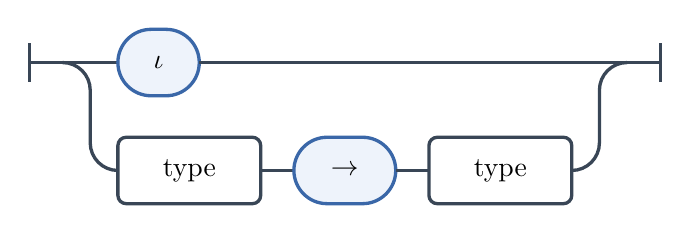
\begin{tikzpicture}[x=1pt, y=1pt]
  \draw[line width=1.2pt, draw=sdgLine, rounded corners=10pt] (8,66) -- (8,52);
  \draw[line width=1.2pt, draw=sdgLine, rounded corners=10pt] (8,59) -- (20,59);
  \draw[line width=1.2pt, draw=sdgLine, rounded corners=10pt] (20,59) -- (40,59);
  \draw[line width=1.2pt, draw=sdgTermLine, fill=sdgTermFill, rounded corners=12pt] (40,47) rectangle (69.4,71);
  \node at (54.7,59) {$\iota$};
  \draw[line width=1.2pt, draw=sdgLine, rounded corners=10pt] (69.4,59) -- (204,59);
  \draw[line width=1.2pt, draw=sdgLine, rounded corners=10pt] (204,59) -- (224,59);
  \draw[line width=1.2pt, draw=sdgLine, rounded corners=10pt] (20,59) -- (30,59) -- (30,20) -- (40,20);
  \draw[line width=1.2pt, draw=sdgLine, fill=white, rounded corners=3pt] (40,8) rectangle (91.6,32);
  \node at (65.8,20) {\textrm{type}};
  \draw[line width=1.2pt, draw=sdgLine, rounded corners=10pt] (91.6,20) -- (103.6,20);
  \draw[line width=1.2pt, draw=sdgTermLine, fill=sdgTermFill, rounded corners=12pt] (103.6,8) rectangle (140.4,32);
  \node at (122,20) {$\to$};
  \draw[line width=1.2pt, draw=sdgLine, rounded corners=10pt] (140.4,20) -- (152.4,20);
  \draw[line width=1.2pt, draw=sdgLine, fill=white, rounded corners=3pt] (152.4,8) rectangle (204,32);
  \node at (178.2,20) {\textrm{type}};
  \draw[line width=1.2pt, draw=sdgLine, rounded corners=10pt] (204,20) -- (214,20) -- (214,59) -- (224,59);
  \draw[line width=1.2pt, draw=sdgLine, rounded corners=10pt] (224,59) -- (236,59);
  \draw[line width=1.2pt, draw=sdgLine, rounded corners=10pt] (236,66) -- (236,52);
\end{tikzpicture}%
}
\end{center}
\end{definition}

\begin{proposition}
任意の$A \in \mathbb{T}$は$\mathbb{B}$の元か$A_1, A_2 \in \mathbb{T}$により一意的に$(A_1 \to A_2)$と表される.
\end{proposition}

\begin{remark}
$A,B,C \in \mathbb{T}$に対して$(A \to (B \to C))$を$A \to B \to C$と表す.
\end{remark}